%
% FH Technikum Wien
% !TEX encoding = UTF-8 Unicode
%
% Erstellung von Master- und Bachelorarbeiten an der FH Technikum Wien mit Hilfe von LaTeX und der Klasse TWBOOK
%
% Um ein eigenes Dokument zu erstellen, müssen Sie folgendes ergänzen:
% 1) Mit \documentclass[..] einstellen: Master- oder Bachelorarbeit, Studiengang und Sprache
% 2) Mit \newcommand{\FHTWCitationType}.. Zitierstandard festlegen (wird in der Regel vom Studiengang vorgegeben - bitte erfragen)
% 3) Deckblatt, Kurzfassung, etc. ausfüllen
% 4) und die Arbeit schreiben (die verwendeten Literaturquellen in Literatur.bib eintragen)
%
% Getestet mit TeXstudio mit Zeichenkodierung ISO-8859-1 (=ansinew/latin1) und MikTex unter Windows
% Zu beachten ist, dass die Kodierung der Datei mit der Kodierung des paketes inputenc zusammen passt!
% Die Kodierung der Datei twbook.cls MUSS ANSI betragen!
% Bei der Verwendung von UTF8 muss dnicht nur die Kodierung des Dokuments auf UTF8 gestellt sein, sondern auch die des BibTex-Files!
%
% Bugreports und Feedback bitte per E-Mail an latex@technikum-wien.at
%
% Versionen
% *) V0.7: 9.1.2015, RO: Modeline angepasst und verschoben
% *) V0.6: 10.10.2014, RO: Weitere Anpassung an die UK
% *) V0.5: 8.8.2014, WK: Literaturquellen überarbeitet und angepasst
% *) V0.4: 4.8.2014, WK: Initalversion in SVN eingespielt
%
\documentclass[MME,Projekt,english]{twbook}%\documentclass[Bachelor,BMR,ngerman]{twbook}
\usepackage[utf8]{inputenc}
\usepackage[T1]{fontenc}

% TIKZ Configuration
\usepackage{tikz}
\usetikzlibrary{shapes.geometric, arrows}
\tikzstyle{startstop} = [rectangle, rounded corners, minimum width=6cm, minimum height=1cm,text centered, draw=black, fill=red!30]
\tikzstyle{io} = [trapezium, trapezium left angle=70, trapezium right angle=110, minimum width=6cm, minimum height=1cm, text centered, draw=black, fill=blue!30]
\tikzstyle{process} = [rectangle, minimum width=6cm, text width=6cm, minimum height=1cm, text centered, draw=black, fill=orange!30]
\tikzstyle{decision} = [diamond, minimum width=3cm, minimum height=1cm, text centered, draw=black, fill=green!30]
\tikzstyle{arrow} = [thick,->,>=stealth]

%
% Hier biblatex & Biber konfigurieren; Vergessen Sie nicht, dass Sie biber verwenden müssen um eine Bibliothek zu erzeugen
%
\usepackage[backend=biber, style=numeric]{biblatex}
\addbibresource{Literature.bib}

%
% Bei Bedarf bitte hier die Syntax-Highlightings anpassen
%
\usepackage[final]{listings}
\lstset{captionpos=b, numberbychapter=false,caption=\lstname,frame=single, numbers=left, stepnumber=1, numbersep=2pt, xleftmargin=15pt, framexleftmargin=15pt, numberstyle=\tiny, tabsize=3, columns=fixed, basicstyle={\fontfamily{pcr}\selectfont\footnotesize}, keywordstyle=\bfseries, commentstyle={\color[gray]{0.33}\itshape}, stringstyle=\color[gray]{0.25}, breaklines, breakatwhitespace, breakautoindent}
\lstloadlanguages{[ANSI]C, C++, [gnu]make, gnuplot, Matlab}

%Formatieren des Quellcodeverzeichnisses
\makeatletter
% Setzen der Bezeichnungen für das Quellcodeverzeichnis/Abkürzungsverzeichnis in Abhängigkeit von der eingestellten Sprache
\providecommand\listacroname{}
\@ifclasswith{twbook}{english}
{%
    \renewcommand\lstlistingname{Code}
    \renewcommand\lstlistlistingname{List of Code}
    \renewcommand\listacroname{List of Abbreviations}
}{%
    \renewcommand\lstlistingname{Quellcode}
    \renewcommand\lstlistlistingname{Quellcodeverzeichnis}
    \renewcommand\listacroname{Abkürzungsverzeichnis}
}
% Wenn die Option listof=entryprefix gewählt wurde, Definition des Entyprefixes für das Quellcodeverzeichnis. Definition des Macros listoflolentryname analog zu listoflofentryname und listoflotentryname der KOMA-Klasse
\@ifclasswith{scrbook}{listof=entryprefix}
{%
    \newcommand\listoflolentryname\lstlistingname
}{%
}
\makeatother
\newcommand{\listofcode}{\phantomsection\lstlistoflistings}

% Die nachfolgenden Pakete stellen sonst nicht benötigte Features zur Verfügung
\usepackage{blindtext}

%
% Einträge für Deckblatt, Kurzfassung, etc.
%
\title{Physicalisation of Upper Airway \\Models for Applications in Respiratory \\Research}
%\author{Titel Vorname Name, Titel}
%\studentnumber{XXXXXXXXXXXXXXX}
\author{Leonhard Hauptfeld}
\studentnumber{me21m003}
\supervisor{Richard Pasteka}
%\supervisor[Begutachter]{Titel Vorname Name, Titel}
%\supervisor[Begutachterin]{Titel Vorname Name, Titel}
%\secondsupervisor{Titel Vorname Name, Titel}
%\secondsupervisor[Begutachter]{Titel Vorname Name, Titel}
%\secondsupervisor[Begutachterinnen]{Titel Vorname Name, Titel}
\place{Wien}
\kurzfassung{\blindtext}
\schlagworte{Schlagwort1, Schlagwort2, Schlagwort3, Schlagwort4}
%\outline{\blindtext}
\keywords{Keyword1, Keyword2, Keyword3, Keyword4}
%\acknowledgements{\blindtext}

\begin{document}

\maketitle

\chapter{Introduction}

\section{Vision}

Upper airway modelling is a relatively new field and is being widely researched nowadays. Among other research, it could even gain relevance with regards to the recent proliferation of the SARS-CoV-2 variants, as the virus increasingly attacks the upper airways\cite{omicronairways}. Understanding and modelling these passages provides insight into their functionality and the effect of diseases. Aside from maintaining the confidentiality of volunteer CT data, there are also no significant ethical concerns with this sort of modelling, unlike in the case of animal testing. Some work has already been done in this project by a student group - the previous “Upper Airway Model” project succeeded in providing a 3D airway model from a single CT scan that can be rapidly manufactured for testing. However, the variability of human anatomy through age and other factors means that only one model is not nearly enough to account for the wide range of possible airway configurations and as such the process had to be altered and refined to allow for rapid creation of new manufacturable airway models to consequently ensure more meaningful results through a broader range of tested models.

\section{Goal of the project}

The goal of the project was to turn a digital model of an upper airway system to a physical one for testing.
The physical model was to be tested using pressurized air and measurements taken that prove soundness and air-tightness of the model.
For the physical testing, hardware and software that could take those measurements needed to be developed.
To facilitate process usability, a document explaining the streamlined process was to be created.
\section{State of the art}

Some upper airway models exist at UAS Technikum Wien for researching mask effectiveness, inhaler efficiency and other respiration related topics.
No guidelines or processes for development of models exists or was accessible for the purposes of this research, therefore none is assumed to exist.

\section{Analysis}

The lack of a more universally applicable and documented process needs to be addressed. In addition, development of an in-house
measurement device with accompanying custom software could benefit research by removing the need for expensive external equipment. Furthermore,
such a device could be customized to the needs of research conducted at UAS Technikum.

\chapter{Materials and Methods}

The main processes are split into those required to accomplish creating a model for physical testing ("Physicalisation") and those necessary for
printing it. The resulting processes then need to be documented. Finally, a device and accompanying software for physical measurements are developed.

\section{Requirements and approaches for a physicalisation process}

\subsection{Requirements}

The process of editing the mesh for physicalisation needs to keep to a few key requirements.

\begin{itemize}
	\item \textbf{Accuracy} | The resulting mesh needs to be true to the original airways with regards to analysis.
	\begin{itemize}
		\item The air-facing parts of the resulting mesh for printing needs to match the air-facing parts of the original mesh.
		\item Parts that don't interact with airflow (for example, the outer wall) can be modified as required.
	\end{itemize}
	\item \textbf{Usability} | The process needs to be as easy to use as possible by someone with little previous knowledge.
	\begin{itemize}
		\item Keep number of steps to the minimum necessary
		\item Document common errors and anomalies with ways to resolve them
	\end{itemize}
	\item \textbf{Universality} | The process needs to be as universally applicable as can be.
	\begin{itemize}
		\item The basic principles should be applicable to the majority of airways.
		\item There cannot be a catch-all solution to every airway model. Universality is restricted in that regard.
	\end{itemize}
\end{itemize}

\subsection{Evaluating software}

The process will need to make use of one more applications to aid in mesh manipulation.
The amount of required software should be kept to a minimum to avoid the user needing to install it all in
addition to keeping it updated.

Software is evaluated based on a few key criteria:
\begin{itemize}
	\item \textbf{Ease of Use} | An overall impression of the UI, how "fool-proof" the software is, how many errors it allows, how fast it can be learned, etc.
	\item \textbf{Functionality} | How many tools the software provides, how useful they are for this application and how well they work
	\item \textbf{Availability} | Whether the software is free to download, free for academic purposes or requires a purchase. Additionally, being Open Source is a bonus due to the guaranteed continued availability.
	\item \textbf{Automatability} | A minor point - how automatable the software is through scripting or similar. Some processes could eventually be automated through this.
\end{itemize}

The evaluated software will be Autodesk Fusion 360, Blender and OpenSCAD.

\newpage

\subsection{Process development}

The process is to be developed by first identifying all the required subprocesses and then working out a
basic working routine for each. The basic routine is then evaluated based on the process evaluation critera - if they
are not deemed sufficiently fulfilled (e.g. a significant deviation from the original mesh) the existing steps are
then refined by experimenting with new tools and methods. The new steps are then again evaluated. This repeats until
all the criteria are sufficiently fulfilled and the process is worked out (Fig. \ref{phys-process-dev}).\\

\begin{figure}[!htbp]
	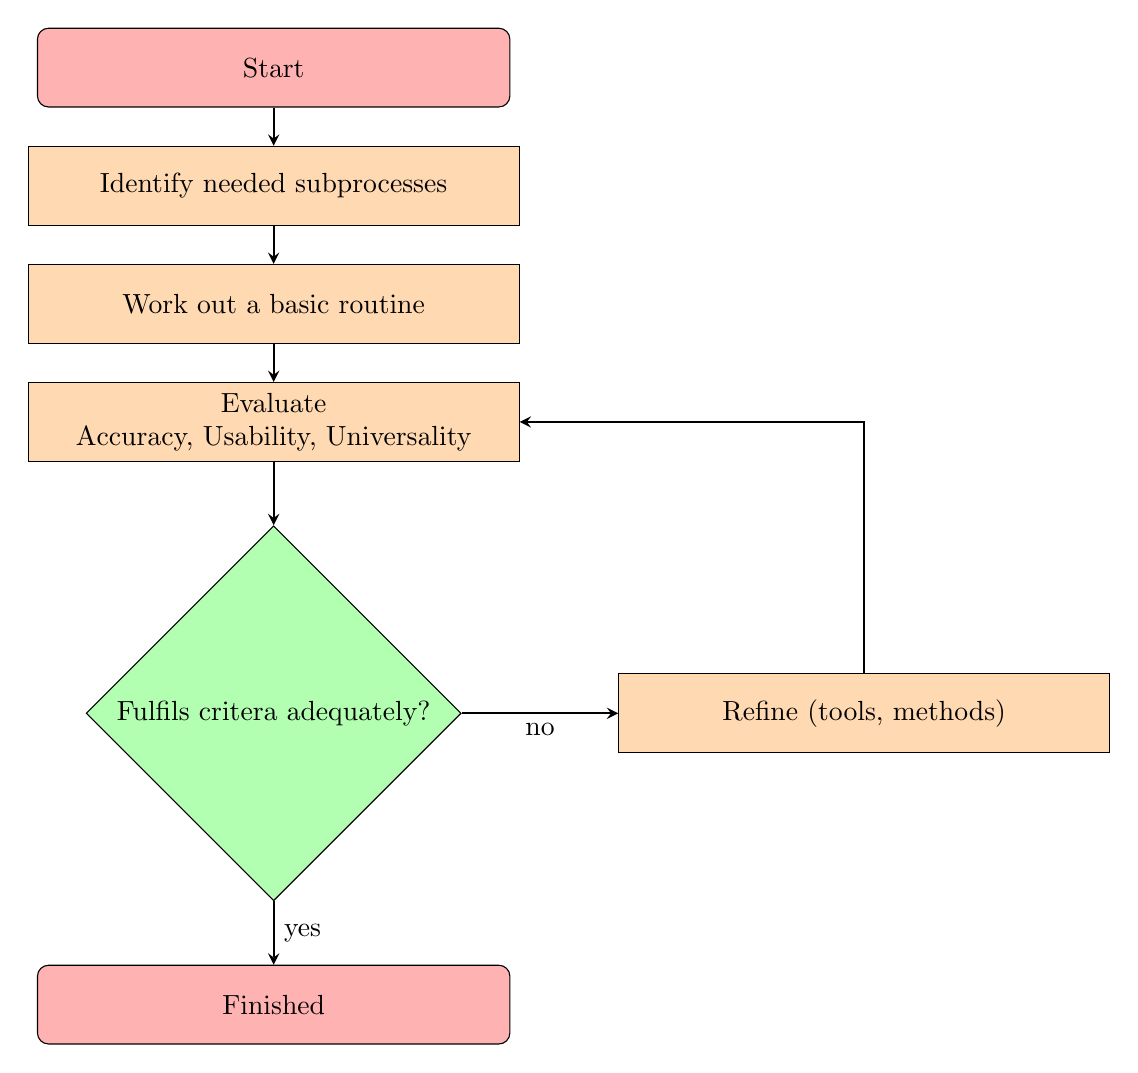
\begin{tikzpicture}[node distance=1.5cm]
		\node (start) [startstop] {Start};
		\node (subpro) [process, below of=start] {Identify needed subprocesses};
		\node (basic) [process, below of=subpro] {Work out a basic routine};
		\node (eval) [process, below of=basic] {Evaluate\\Accuracy, Usability, Universality};
		\node (crit) [decision, below of=eval, yshift=-2.2cm] {Fulfils critera adequately?};
		\node (refine) [process, right of=crit, xshift=6cm] {Refine (tools, methods)};
		\node (finish) [startstop, below of=crit, yshift=-2.2cm] {Finished};
	
		% Sequential Flow
		\draw [arrow] (start) -- (subpro);
		\draw [arrow] (subpro) -- (basic);
		\draw [arrow] (basic) -- (eval);
		\draw [arrow] (eval) -- (crit);
		% Eval decision
		\draw [arrow] (crit) -- node[anchor=north] {no} (refine);
		\draw [arrow] (crit) -- node[anchor=west] {yes} (finish);
		\draw [arrow] (refine) |- (eval);
	\end{tikzpicture}
	\caption{Physicalisation process development}\label{phys-process-dev}
\end{figure}

\section{Requirements and approaches for a printing process}

\subsection{Requirements}

The requirements to the printing process are broadly the same as to the mesh process - Accuracy, Usability and Universality.
Accuracy in 3D printing pertains to how accurate the printed airway model will be compared to the provided mesh.
Universality is additionally relevant when it comes to the wide variety of available 3D printers and how well the printing process
works for them. The usability concerns remain the same. As an additional requirement, the printed model
will need to be air tight.

\subsection{Process development}

As most of the printing process is automated, the relevant user input is in material choice and printing settings.
Different materials and printing settings have to be tried and the printed results evaluated - again with regards to accuracy and universality.\\

Materials to be evaluated:
\begin{itemize}
	\item \textbf{PLA} | Brittle but easy to work with, can be printed on any FDM printer
	\item \textbf{ABS} | Stronger and more flexible but requires more advanced FDM printers and is prone to deforming during print
	\item \textbf{TPU} | Strong and flexible, provides good sealing surfaces, hardest to print of all three
\end{itemize}

Settings to be evaluated:
\begin{itemize}
	\item \textbf{Layer Height} | Height of an individual FDM layer, 0.1, 0.15 or 0.2mm
	\item \textbf{Supports} | Where to generate support struts for model overhangs
	\item \textbf{Model Placement} | Where to place and how to orient the model on the print bed
\end{itemize}
All other settings are too specific to individual printer models to be set with any certainty. The prints
will be tested on an Ultimaker 2+.

Models are printed using a subset of settings and evaluated based on the above-mentioned criteria. If a printed model
does not pass the criteria (e.g. is not air tight or too brittle) the settings are changed and the model is re-printed to be evaluated again.
If a printed model passes muster, the settings are noted down for documentation.

\section{Documentation of processes}

Both the finalized mesh modification and printing processes are to be documented in an easily accessible
form with picture guidance. This resulting guide document needs to conform to the same usability requirement
as the processes themselves.

\section{Developing and evaluating hardware and software for measurements}

\subsection{Hardware}

For measurements of airflow and pressure in physical airway models, a device needs to be created
that can take these measurements. The requirements are as folllows:

\begin{itemize}
	\item \textbf{Flow Measurements} | Take airflow measurements from 2 or more sensors on a typical human breathing scale (5-10 l/min)
	\item \textbf{Pressure Measurements} | Take air pressure measurements from 2 or more sensors on a typical human breathing scale (0-10kPa)
	\item \textbf{Transmission} | Transmit those signals in a timely and reliable manner to a computer
\end{itemize}

An appropriate microcontroller and sensors that work within the specified ranges need to be selected.
In addition, a method of data transmission needs to be worked out that adheres to the timeliness and reliability principles.

\subsection{Software}

The software needs to be able to handle the incoming data from the measurement device and log it
to storage reliably. Additional functionality could include display and analysis but these features are not required.

A language and/or framework that can handle the requirements and is maintainable needs to be selected and the
program implemented.

\newpage
\chapter{Results}

\section{Novel mesh editing processes}

\subsection{Software Evaluation}
\begin{table}[h]
	\caption{Mesh software evaluation}\label{mse}
	\begin{tabular}{|p{0.15\textwidth}|p{0.2\textwidth}|p{0.2\textwidth}|p{0.2\textwidth}|p{0.2\textwidth}|}
	\hline
	\textbf{Software}   & \textbf{Ease of Use}                                                                      & \textbf{Functionality}                                                                           & \textbf{Availability}                    & \textbf{Automatability}                  \\ \hline
	Fusion 360 & Centered around usability. Friendly user interface, easiest CAD software.        & Strong CAD and Mesh functionality, centered around physical models.                     & Free for Education, Proprietary & None                            \\ \hline
	Blender    & Medium usability.Lots of tutorials are available, can be learned in a few days. & Primarily used for CGI. Some 3D printing tools are available. Wide array of mesh tools. & Free, Open Source               & Python Interface                \\ \hline
	OpenSCAD   & Not easy. Models are created in custom scripting language. Steep learning curve. & CAD modelling only. Almost limitless programmable functionality.                        & Free, Open Source               & Completely (Models are Scripts) \\ \hline
	\end{tabular}
\end{table}

Blender was chosen for mesh manipulation and OpenSCAD for CAD modelling of required additional parts. Blenders powerful mesh editing tools
and OpenSCADs versatility in addition to both of these applications being Open Source were key decision points.

\newpage
\subsection{Hollowing}

The Blender "Solidify" modifier was used to create an airway mesh with a wall. By specifying a negative value for wall thickness,
the walls were created towards the outside of the airways and thus did not narrow the inner airway paths (Fig. \ref{blender-hollowing}) Inside geometry was ignored by the tool,
so inside features like tonsils were unaffected. 

\begin{figure}[!htbp]
	\centering
	\includegraphics[width=1\linewidth]{images/blender-hollowing}
	\caption{Hollowing in Blender}\label{blender-hollowing}
\end{figure}

\subsection{Cutting into segments}

Two different Blender tools for mesh slicing - the knife and bisect tools - were tested. The bisect tool was used for the final process.

\subsubsection{Knife Tool}

The knife tool was the first method attempted for cutting airway meshes into segments. It is a fairly advanced tool
that allows projecting 2D shapes onto the 3D geometry to create cut points. While powerful, this tool requires many steps
to use - 2D geometry needs to be created and the projection needs to be adjusted accordingly. Since separation of airway segments requires
just a cut along a plane, this tool failed on the Usability criterion.

\subsubsection{Bisect Tool}

The bisect tool is a fairly straightforward tool in Blender to cut a mesh along an infinite plane. It is extremely
intuitive to use (dragging a line over the mesh). The tool itself only creates the vertices and edges along the mesh - in addition, the mesh
needs to be separated. This is accomplished using the "Rip" tool. (Fig. \ref{blender-bisect})

\begin{figure}[!htbp]
	\centering
	\includegraphics[width=.5\linewidth]{images/blender-bisect}
	\caption{Bisecting in Blender}\label{blender-bisect}
\end{figure}

\section{Parametric connector system}

Once an airway model is hollowed and cut into segments, there needs to be a way to connect the different segments after printing
in an air-tight way. Additionally, there need to be measurement ports for flow (input/output points of the model) and pressure.

These requirements are accomplished by a universal connector system that consists of adapter plates and features. Adapter plates
are parametric round, flat surfaces with a large center hole on the model. These are attached at the end of airway segments and
allow them to be connected to each other. Adapter plates can also be placed on the side of a model.

Apart from to each other, adapter plates can also be connected to features. Features are adapter plates that have certain attachments
that fulfil a specific purpose like providing a spot to attach a ventilator tube or pressure sensor. The core concept of the system
is that adapter plates and features generated with the same parameters are always compatible with each other. As long as a model has
the parameters of its adapter plates documented, matching features can be generated for it.

The adapter plates and features are implemented in OpenSCAD scripts.

\begin{figure}[!htbp]
	\centering
	\includegraphics[width=.5\linewidth]{images/connector-system}
	\caption{Illustration of the connector system}\label{connector-system}
\end{figure}

\newpage
\subsection{Adapter plate}

Adapter plates are simple discs of a certain thickness with a large centered hole (Fig. \ref{adapter-plate}). They can be generated either as the disk
for attachment to a mesh or in a drill form that is used for inserting appropriately spaced holes into an existing flat surface on a mesh.

\begin{figure}[!htbp]
	\centering
	\includegraphics[width=.3\linewidth]{images/default_adapter.png}
	\caption{Adapter plate}\label{adapter-plate}
\end{figure}

\newpage

They are customizable through the following parameters:

\begin{table}[h]
	\caption{Adapter plate parameters}\label{mse}
    \centering
	\begin{tabular}{|p{0.18\textwidth}|p{0.18\textwidth}|p{0.1\textwidth}|p{0.4\textwidth}|}
    \hline
        Name & Variable & Default & Description \\ \hline
        Diameter & d & 20 & Either the inner or the outer diameter of the adapter plate, depending on if adapter\_plate\_id or adapter\_plate\_od is used. \\ \hline
        Height & h & 2 & The thickness of the adapter plate or the length of the drill. \\ \hline
        Spacing & spacing & 2 & Space between screw holes and adapter edges. \\ \hline
        Screw Diameter & screw\_dia & 3 & Diameter of screw holes. It is generally advisable to keep this a bit below the actual screw size for a good fit, e.g. 2.8 for M3 bolts. \\ \hline
        Screw Number & screw\_num & 3 & Number of screw holes evenly distributed across the plate. It is not advisable to drop this number below 3 unless space is tight. \\ \hline
    \end{tabular}
\end{table}

Since default values for all the parameters are provided, only differing values have to be documented for adapter plates on models.

\subsubsection{Attaching an adapter plate to a segment end}

After cutting a segment of the airway mesh, the geometry is left open (Fig. \ref{blender-bisect}). An adapter plate needs to be attached
and this open geometry closed (made uniform) to allow for error-free 3D printing.

The diameter of the open airway segment is measured. Then, an adapter plate with the appropriate inner diameter is generated. It is moved
into position to align with the cut and joined with the surrounding mesh. The exact process with images can be found in the guide document.

This process went through several iterations of refinement, reducing the number of steps and most importantly automating
the most time-intensive step (selecting the specific mesh for removal) by use of a built-in Blender tool. This also cut down
dramatically on the number of user errors that could occur, since the manual selection of specific mesh also required the most manual
precision.

\subsubsection{Attaching an adapter plate to a segment side}

For an adapter plate surface on the side of an airway segment, the Blender knife tool is used. Unlike in cutting of airway segments,
this process requires the precision of that tool. A circular segment is cut out of the side of the mesh and brought to be vertically
level. A "drill" adapter plate object is generated and boolean combined with the airway mesh to create matching screw holes for attachment
of a feature. The exact process with images can be found in the guide document.

This process went through one major iteration where the process wasn't made easier for the user but the resulting mesh ended up
far cleaner and easier to 3D print by removing jagged edges on the corners of the flat surface.

\subsection{Features}

There are two features that can be generated for adapter plate attachment points - air hose and vent tube connectors.

\begin{itemize}
	\item \textbf{Air hose connectors} are a design that allows for attachment of any size air hose, for example to attach a small diameter hose for a pressure sensor.
	\item \textbf{Vent tube connectors} are specifically made to provide a tight fit for standard 21/22mm ventilator tubing.
\end{itemize}

\begin{figure}[!htbp]
	\centering
	\includegraphics[width=.5\linewidth]{images/features.png}
	\caption{Air hose (left) and vent tube (right) connector features}\label{features}
\end{figure}

\section{Printing process}

Printing settings were evaluated by modelling and attempting to print trachea and larynx/pharynx of the model with the identifier "0190673870\_16a\_M". Only one set of settings was tried and provided adequate results. Only one material was tried (PLA).

A layer height between 0.15mm and 0.2mm is acceptable for printing an airway model. The increased speed from these layer heights dramatically
cuts down printing times and the added precision provided by printing with lower layer heights provides no advantages considering
the low resolution of the underlying CT data.

Support material has to be generated everywhere. With a quality 3D printer, the overhang angle at which such material is generated
can be reduced. Due to the model being split up into many segments, it is not a problem to remove support material from inside the airways
with a screwdriver or long, slim pair of pliers.

Models should be placed with one of their flat adapter plates facing the buildplate. This provides maximum adhesion to the buildplate.
Whichever plate facing down requires less support material is to be preferred.

\begin{figure}[!htbp]
	\centering
	\includegraphics[width=.5\linewidth]{images/larynx_pharynx.png}
	\caption{Printed larynx/pharynx of 0190673870\_16a\_M}\label{larynx_pharynx}
\end{figure}

\section{UAM Guide - Guide document for airway work}

The finalized processes for physicalising and printing were documented in an appealing format by use of the
tool mkdocs. Step-by-step guides with pictures written in markdown are converted a full HTML page that can be considered
a wiki of upper airway modelling. The guide can also be exported as a PDF document.

Error states were documented in additional "info boxes" that are inserted into the guide whenever appropriate to warn
of potential common errors or additional information such as useful tools or suggested procedures.

\begin{figure}[!htbp]
	\centering
	\includegraphics[width=.8\linewidth]{images/uam-guide.png}
	\caption{UAM Guide}\label{uam-guide}
\end{figure}

\section{UAM Thing - A thing for airway measurements}

UAM Thing is a sensor platform that supports four MPX5100/MPX5010 pressure sensors (P1-P4) and four SFMxxxx flow sensors (Q1-Q4). It transmits
data via MQTT to a computer that can log the data via a tool of choice.

\subsection{Choosing components}

The Espressif ESP32 was chosen as the microcontroller at the heart of the device. It is fast enough to handle more concurrent
operations than this project requires, has a crash-resistant real time operating system and extensive connectivity via WiFi, two I2C
controllers and 2 ADCs with 6 channels each.

For a pressure sensor that could provide readings in the required ranges, the MPX5xxx series was chosen. The MPX2xxx series was evaluated but
the need for an external amplification circuit would've greatly increased circuit complexity. The MPX5xxx provides internal amplification
for an output level between 0.2V and 4.7V. This would only require a voltage divider for the ESP32s maximum input level of 3.3V.

As a flow sensors, the SFMxxxx series was chosen due to it being made for ventilation devices and therefore supporting all the
common tubing connections and measuring ranges. Its 5V logic level would require level shifting to the ESP32s 3.3V and the inability
to change I2C adress on the SFM3xxx series meant multiplexing of the I2C bus would be required.

\subsection{Developing circuit board and case}

\subsubsection{SFMxxxx}

Due to the SFM3xxx series having a fixed I2C address (0xH40), the choice was to either use both of the ESP32s hardware I2C drivers,
software I2C or an I2C multiplexing chip. Since software I2C is less reliable than the hardware driven equivalent and level
shifting had to be done anyway, the multiplexing method was chosen. A breakout board based on the TCA9458A multiplexer chip
is connected to all four SFM sensor channels. The ESP is connected to this multiplexer via one of its hardware I2C drivers. The ESP
would have to continually iterate over all connected channels to get new measurement values. Since the I2C bus on all of these devices
can operate at a high 400kHz and SFM sensors have a response time of 1ms (1kHz), this wouldn't impede sampling rate in any way. In addition,
the TCA9458A handles level shifting between 3.3V and 5V. All I2C lines are pulled up to the appropriate voltage through 10kOhm resistors.

The SFM sensors feature a unique pad connector for which a clamp has to be manufactured that attaches to the sensor. A design from
the online repository Thingiverse (4924085 by "nicksears") was used as it could be manufactured with readily available pogo pins. The other
end of the connection was to be made through 4 pin JST-XH connectors. The heating lines on the sensor are left unconnected, as the
evaluations within the scope of this project did not require working with very humid air.

\subsubsection{MPX5xxx}

The MPX sensors provide a typical output voltage range from 0.2V to 4.7V. This was halved by use of a voltage divider (R1=100kOhm, R2=100kOhm).
The resulting output voltage would therefore range from 0.1V to 2.35V. Set to 11dB of attenuation, the
ESP32s ADC could reliably read voltages from 150mV to 2450mV (Fig. \ref{esp-adc}). Below 150mV, the ADC reads zero - the pressure ranges of 0 to 0.33kPa (MPX5010)
and 0 to 3.33kPA (MPX5100) are therefore unreadable.

\begin{figure}[!htbp]
	\centering
	\includegraphics[width=.8\linewidth]{images/esp-adc.png}
	\caption{ESP32 ADC curve at 11dB attenuation}\label{esp-adc}
\end{figure}

The sensors are connected via 6-pin 2.54mm pin headers. Since the MPX5100 and MPX5010 both share the same pin arrangement, they can
be used interchangeably. This configuration is fully supported.

Smoothing capacitors are used for the power supply and each ADC channel as recommended by the application circuit in the MPX datasheets
to provide more consistent results.

\subsubsection{Hardware}

The schematic was drawn up in KiCads eeschema and a hand-solderable board was created in KiCads pcbnew. A 3D model of this
circuit board was then imported into OpenSCAD, where a case was modelled around it. The case features descriptions of the sensor ports
and a little guide graphic to prevent insertion of the MPX sensors in the wrong orientation.

\begin{figure}[!htbp]
	\centering
	\includegraphics[width=.5\linewidth]{images/uam-thing-case.png}
	\caption{UAM Thing case}\label{uam-thing-case}
\end{figure}

\subsection{Implementing firmware}

MQTT was chosen as the protocol for transmission of data. MQTT is based on publishing data in channels identified by strings and
is simple, fast and widely implemented for all kinds of programming languages.

On Startup, the ADC channels are configured and the internal calibration values loaded to ensure correct readings from the MPX sensors.
The SFM sensors are contacted through I2C and their serial as well as calibration values read. SFM sensors that don't respond on
initialization are excluded from any further querying to save on unneccessary communication attempts.

The ESP32 then creates a WiFi network with a name configured in the firmware. As soon as a computer connects, it attempts
to connect to an MQTT server on that computer. Publishing of sensor data on that server then starts immediately.

Two tasks in the ESP32's RTOS then run periodically every 200ms.

\begin{itemize}
\item The FlowSensors task iterates through all connected SFM sensors
and reads their values. The values are converted to slm and reported on the MQTT channel "/uam-thing/<device-id>/flow/<sensor-id>". Additionally,
any communication with SFM sensors is error checked by means of CRC8 values to ensure accurate reporting of sensor data.

\item The PressureSensors task iterates over all ADC1 channels and reads the raw value of each. Using the internal calibration of
the ESP32, the readings are converted to voltages where they are converted to kPa. The ratio is determined by whether the port is
set to be an MPX5010 or MPX5100 sensor in the firmware. The kPA values are then reported on the MQTT channel "/uam-thing/<device-id>/pressure/<sensor-id>".
\end{itemize}

\subsection{Preliminary testing}

A prototype UAM Thing was constructed.

To establish plausbility of pressure sensor readings, an MPX5100 sensor was attached to a pressure source set to 0.5 bar or 50kPa.
The sensor readings read between 49 and 52kPa. As the pressure source manometer was not highly accurate, this was determined to be
acceptable to establish basic plausbility of sensor readings. A separate evaluation against a professional pressure measurement
device would need to be performed to perform a full calibration.

Since the SFM sensors are pre-calibrated and communicate via I2C, a basic plausibility test was not considered necessary.

\begin{figure}[!htbp]
	\centering
	\includegraphics[width=.6\linewidth]{images/pressure-test.png}
	\caption{Pressure testing setup}\label{pressure-test}
\end{figure}

\newpage

\section{UAM Workbench - Software for airway work}

Creation of airway models is a multimodal environment, where CT segmentation, CAD, modelling and datalogging tools have to be used.
To create a data structure that could house all that data and bind it to the context of one model, a software called UAM Workbench
was prototyped. This software would store all metadata pertaining to an airway model in a JSON file. Remote interfaces to 3D Slicer
and Blender were prototyped to allow the software to aid in tasks within these programs and help it manage their complex file structure.
In addition, it was to contain a built-in MQTT server for UAM Thing and a tool for logging and displaying its sensor data.

This app would be developed using the Tauri development framework to ensure a modern user experience.

Basic management of the file structure as well as prototype interfaces to Blender and UAM Thing were achieved. The tool exists in
a little showcase format but is, as of submission (28.9.2022), not production-ready.

\begin{figure}[!htbp]
	\centering
	\includegraphics[width=.6\linewidth]{images/uam-workbench.png}
	\caption{UAM Workbench - Welcome Screen}\label{uam-workbench}
\end{figure}

\section{Evaluation of entire ecosystem}

To evaluate the entire ecosystem (creation process, connector system, printing process \& UAM Thing) a model of the dataset
"0190673870\_16a\_M" was constructed and a trachea and larynx/pharynx printed. The trachea had vent tube connector features attached at both ends
and an air hose connector feature for 6mm inner diameter tubing attached on the side. No gaskets or other sealing methods were used between adapter plates and features.

An SFM3300 flow sensor at the inlet was connected to port Q1 of the UAM Thing, another SFM3300 sensor was attached at the outlet of the trachea
and to port Q2 of the UAM Thing. An MPX5010DP pressure sensor was connected to port P1 of UAM Thing and a tube was connected between the side feature
of the trachea and the positive pressure input. Figures \ref{eval-setup} and \ref{eval-setup-irl} illustrate this setup.

\begin{figure}[!htbp]
	\centering
	\includegraphics[width=.6\linewidth]{images/eval-setup.png}
	\caption{Ecosystem evaluation - Schematic}\label{eval-setup}
\end{figure}

\begin{figure}[!htbp]
	\centering
	\includegraphics[width=.6\linewidth]{images/eval-setup-irl.jpg}
	\caption{Ecosystem evaluation - Setup}\label{eval-setup-irl}
\end{figure}

Data was logged for a 25 second period while flow was periodically increased up to a point of 300 slm as measured by the inlet sensor Q1. A significant
difference in flow between Q1 and Q2 would indicate a leak.

\begin{figure}[!htbp]
	\centering
	\includegraphics[width=.8\linewidth]{images/eval-result.png}
	\caption{Ecosystem evaluation - Result}\label{eval-result}
\end{figure}

The variance in slm between Q1 and Q2 is negligible, on the order of 1slm. No significant leaks were observed. The pressure sensor remained mostly idle,
only showing 1kPa on occasion when flows over 120 slm were present.

\chapter{Discussion}

\section{Processes and ecosystem evaluation}

Overall, the new processes and guide documents proved to be a success, as they were used quite extensively while conducting
this very research. Error rates and modelling times were gradually reduced overall, though a proper case study about this
including people without prior experience would have to be conducted to say this for certain.

The result in the ecosystem evaluation came unexpected, as a leak without any sealing measures was expected. The adapters performed
better than expected, which might be attributable to their large surface area and the clamping force of the screws that hold them together. Whether
they hold up in higher pressure scenarios would need further evaluation.

\section{Shortcomings and possible improvements of UAM Thing}

\begin{itemize}
	\item A printed circuit board would provide a more robust electrical foundation and cut down on soldering work
	\item The pin headers proved to be insufficient in supporting the weight of the MPX sensors and attached tubing, eventual failure is probable.
		  They could be supported through their own screw holes with a more advanced case design.
	\item Similarly, the JST connectors could be swapped for a sturdier alternative like DIN plugs. JST connectors are rated for around 10.000 cycles.
	\item More calibration work has to be done to ensure accuracy of the MPX sensors especially
	\item Since the device is powered off USB, a more stable 5V supply voltage would be advantageous to prevent crashes of the SFM sensors and ensure accuracy of the MPX sensors. A boost converter could accomplish this.
\end{itemize}
\section{Further process development}
\begin{itemize}
	\item The physicalisation process needs to be trialed with more complex and non-uniform meshes. Some strange errors can occur in those cases,
		  for which resolutions should be documented.
	\item More printing materials and technologies (SLA) need to be trialed with airway models.
\end{itemize}

\newpage
\chapter{References}

\printbibliography[heading=none]

\clearpage
% Das Abbildungsverzeichnis
\listoffigures

% Das Tabellenverzeichnis
\listoftables

% Das Quellcodeverzeichnis
\listofcode

\end{document}
